\chapter{Directed Graphs}

There have been some issues with teaching mathematics lately, and most of those issues have come about from the lack of certain foundational information that we build up from. There are too many people that think math is the study of numbers, and so it would be good to dispel this view, give a real overview of mathematics, and provide intuitive, rational, and practical discussions as we go.

All of this said, philosophy is paramount to understanding mathematics and science, but we are specifically going to work with understanding some basics through graphs.

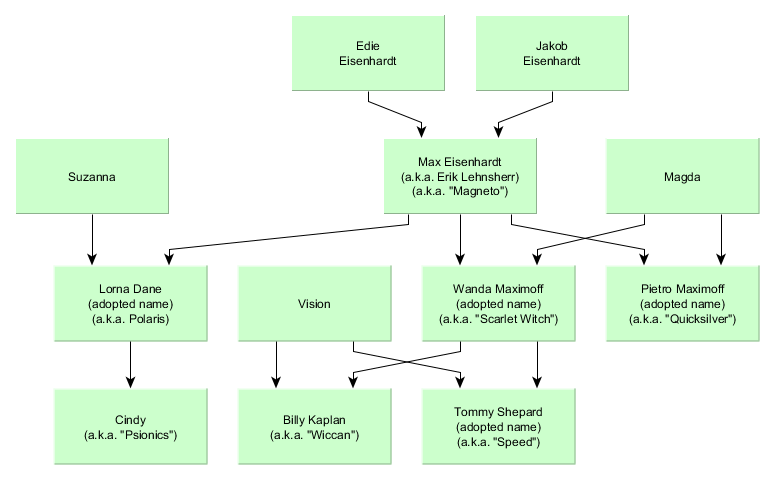
\includegraphics[scale=0.55]{01/XMenAvengersFamilyTree.png}

Looking at the directed graph that I provided, this graph relates parents to their biological children. You can see that Magneto was the father to Polaris, to Scarlet Witch, and to Quicksilver. We consider the relationships that are described by the graph:

\begin{itemize}
    \item Child -- identified as those next people by following the arrows
    \item Parent -- identified by following the arrows to the previous people
    \item Descendant -- identified as any person that can be reached by following arrows directly
    \item Ascendant -- identified as any person that can be reached by following arrows backwards
\end{itemize}

Let's look at another directed graph. This graph is a graph of people that follow each other on Twitter.

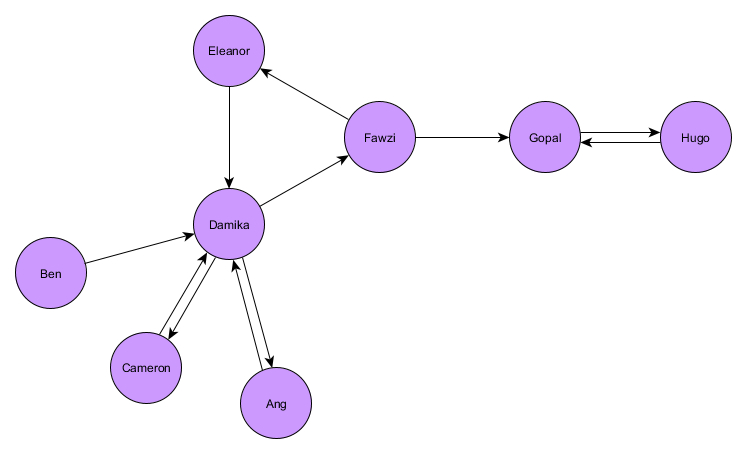
\includegraphics{01/FollowersOnTwitter.png}

We have Hugo following Gopal and Gopal following Hugo, as represented by two arrows, one going each way between the two. However, it's also the case that there are those that follow a person without being followed back. For instance, Ben follows Damika, but Damika is not following Ben back. 

There is also a cycle in the graph. We have that Damika follows Fawzi, and that Fawzi follows Eleanor, and that Eleanor then follows Damika. This forms a cycle between the 3 of them.

In each of this cases, we are defining relationships between things. Mathematics is a useful tool for describing relationships. Later, we will learn exactly how to construct each of these graphs formally, but for now, the idea of using arrows between objects is a notion that should be fairly intuitive for most people.

As far as definitions go, graphs are drawings that relate objects to each other. A \textbf{directed graph} is drawn with arrows, and it denotes one-way relationships. \textbf{undirected graphs} are drawn with lines, and denotes two-way relationships.

Additionally, when talking about Graph Theory, a \textbf{node} is what we are relating, and the \textbf{edge} is the relationship, usually denoted by an arrow.

We can make an undirected graph from a directed graph by removing the arrowheads, such that every edge is understood to go both directions.

We discern graphs from multigraphs, which may have multiple edges leading to the same nodes.

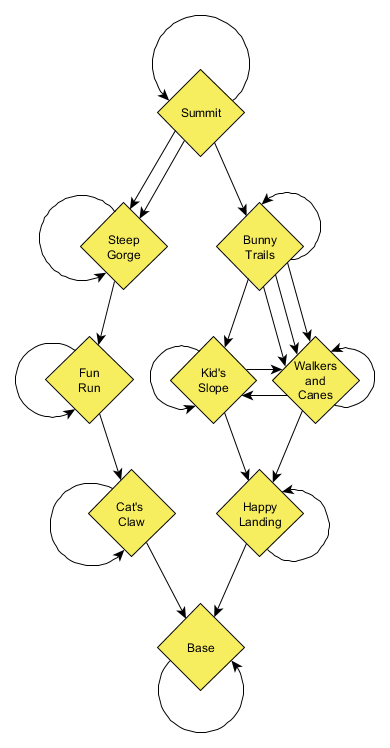
\includegraphics{01/slopes.png}

In this multigraphs, you can see that there are multiple ways to get from the Bunny Trails to Walkers and Canes. The Kid's Slope is right next to Walkers and Canes, and you can walk back and forth between each other, before going down either to Happy Landing.

You will also notice that every single area has a \textbf{loop} that shows that you can get to where you are from where you are. \textbf{Loops} are edges from a node, back to itself. It seems a bit overkill to put this in, but there are some directed graphs where all nodes have loops, some where no nodes have loops, and there are some directed graphs yet where only some nodes have loops.

Loops make sense when describing paths between things. Loops don't make sense when describing parents, since someone cannot be their own parent. Likewise, with Twitter, you don't really follow yourself, so there are no loops. However, if we were discussing 

The only thing to mention is that you cannot walk your way back up the actual slopes themselves. Of course, not pictured, is the ski lift that can take you back to Summit from Base. So, what is represented is the different ways that you can get to each point on your skis (either by skiing or walking). Because there are multiple paths from Bunny Trails to Walkers and Canes (and from Summit to Steep Gorge), it is a directed multigraphs, not a directed graph.

If our only concern was whether or not we could get from one to the next, and not how many paths there were, then we could remove the extra lines:

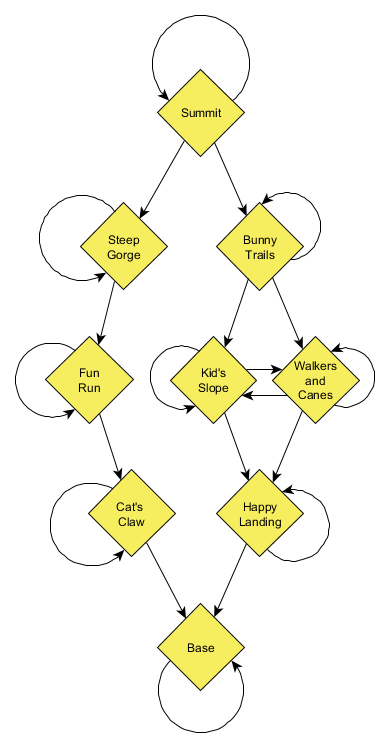
\includegraphics{01/slopes2.png}

Compare the multigraphs of the slopes, to the directed graph of the slopes.

So, directed graphs may only have zero or one edge (i.e. "edge or no edge"), in the same direction, between two nodes, and directed multigraphs may have zero or more edges, in the same direction.

Now, with this in mind, this idea of reachability is important in mathematics, and logic. If we have a directed graph and we only care about reachability, we end up with a \textbf{category graph}.

Because we are only interested in reachability, the category graph for the slopes would look like this:

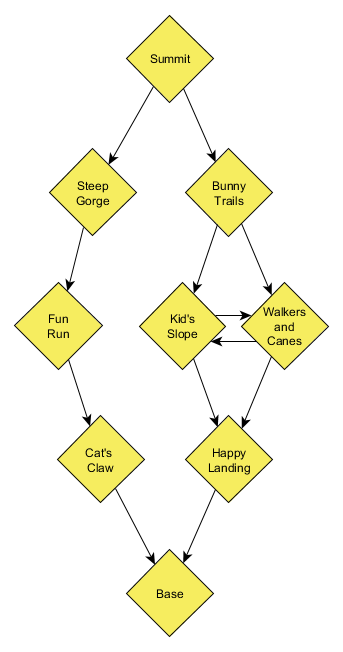
\includegraphics{01/slopes3.png}

In this category graph, we can say that we can reach Bunny Trails from Bunny Trails without having to include the loop itself. Loops are implied in category graphs. Likewise, because a category graph is interested in reachability, we know that we can reach Cat's Claw from Steep Gorge, because we can go through Fun Run to get there.

\chapter{Introduction to Logic}

This is the beginning of understanding logic. Logic starts with this idea of reachability, allowing us to say that, if we are at Steep Gorge, and we can get to Fun Run from Steep Gorge, then we can get to Fun Run.

In logic, when we are talking about reachability, we call it \textbf{deductive closure}, which is the ability to arrive at a \textbf{conclusion} (the target node), based on starting information (the source node), and the relationship (the edge/arrow).

So, let's introduce a category that we usually call a \textbf{rational argument}. We can draw a rational argument in a category graph as well, and work through it.

A \textbf{rational argument} is therefore a collection of \textbf{logical statements} and their relationships.

The usage of the word argument here does not imply some kind of altercation between two people, but is a means to make a claim or justification for why you came to your conclusion.

Let's take a moment, and attempt to make a rational argument. For instance:
\begin{enumerate}
    \item Sprinklers will cause the ground to get wet
    \item Rain will cause the ground to get wet
    \item It rained last night
\end{enumerate}

From this, we have a case where either the first premise or the second premise, can cause our conclusion:

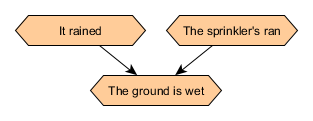
\includegraphics{01/OrCase1.png}

Here, we see the rational argument drawn out. You can see that the phrase, "will cause" has been replaced by an arrow. Often, \textbf{implications} (the logical edges) are due to cause-and-effect relations, but not only is implication much more \textbf{general} (handling many more cases than just cause-and-effect relations), these types of relations don't even form the majority of those that you may use.

Formally, an \textbf{implication} is a relation connecting one \textbf{logical statement} to another logical statement.

However, it's important to notice that the ability for us to discern cause-and-effect relations are probably what gave us the ability to discern other kinds of implications.

Noticing that we have our starting position listed as the 3rd point in our rational argument:

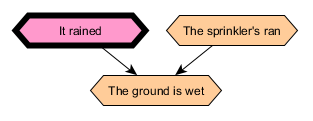
\includegraphics{01/OrCase2.png}

We now look and see what we can reach from there:

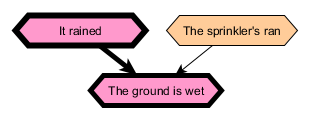
\includegraphics{01/OrCase3.png}

We can \textbf{conclude} that the ground is wet. This extends the information that we have, based only on what was there.

We also note the following: each implication is a \textbf{premise}. Likewise, any \textbf{claim} that a logical statement is \textbf{true} is also a premise. Therefore, the relations and our starting information are all premises of a rational argument.

Where we see an implication, or an arrow between two logical statements, we take that to mean that the target statement must be at least as true as the source statement. That is to say that if the source statement is true, then the target statement must be true. Any time we have an implication, this is what the implication is attempting to give us. 

However, because multiple things may have led to the target being true, that the target is true doesn't mean the source is, instead it may have been because of another cause or implication. Notice that, because the ground is wet, does not mean that it was because the sprinklers were on.

Therefore, the relationship is one way.

Usually, it becomes unwieldy to continually use large sentences in our discussion of rational arguments, so much how our graph has replaced the sentences with numbers, we often use symbols to represent our logical statements.

\begin{itemize}
    \item R -- It has rained
    \item S -- The sprinklers ran
    \item G -- The ground is wet
\end{itemize}

In this case, every time we have one of these letters (R, S, or G), we understand them to stand in place of our sentences above.

Then, we end up with the implications:

\begin{itemize}
    \item $R \to G$
    \item $S \to G$
\end{itemize}

And here, we have the arrows pointing to the target G, in both cases. We can look at this and say in English that ``Either the ground is wet because it rained, \textit{or} because the sprinklers ran''.
\begin{tikzcd}[column sep=0.5cm]
    R \arrow[rd] & \ & \arrow[ld] S \\ 
        & G
\end{tikzcd}

Furthermore, the idea that there are 2 options, even makes sense if they are disconnected from anything. Let's consider this: ``We know that either the sprinklers ran, or that it rained.''. Notice that we didn't include the conclusion: ``that the ground is wet''. In this moment, we don't have to, as we are only going to consider the claim that one of these 2 options must have happened.

Now, if we claim to know that one of two options has happened, and then we claim to know that one didn't, then we are stating that the other happened. In our case, we say that ``the sprinklers didn't run'', but since we know at least one of the two statements happened, then we know that ``it rained'' is the correct statement.

This is another form of \textbf{logical inference}. When we know $R \vee S$ and $\neg R \vdash S$. Let's consider another example of this: Tammy and Sahmail own a car. It's reasonable that one of the two of them are the ones driving it. We are hanging out with Sahmail when we see his car go by. It's reasonable to assume Tammy is driving it.

Logically, we get the statements, ``Tammy is in the car or Sahmail is in the car'' and ``Sahmail is not in the car'' therefore ``Tammy is in the car''.

Furthermore, using our implication from before, we can also state, ``If the car is moving, someone must be driving it'' and ``the car is moving'' therefore ``Tammy is driving''.

So, here, we inferred two different (but related) conclusions using two methods. The first method was \textbf{disjunctive elimination}, which eliminated all other possible cases, and \textbf{modus ponens}, which allows us to conclude via implication. 

Now then, we can 


So, along one branch, we can say that if we know $R$ (``it rained''), and we know that $R \to G$, then we can say that $R, R\to G \vdash G$, which tells us what information we extended ($G$). In some ways it ``feels like'' we have ``computed'' $G$ from $R$ and $R \to G$.

The extended information via this implication is called an \textbf{entailment}. The process of extending our information is a rule of inference. We will learn a few rules of inference (ways to extend our knowledge) as we go, but this one is typically called \textbf{modus ponens}, which is Latin for ``

You'll notice that we have discovered that we can express the connective \textbf{or} in logic. In order to understand it from the information that we gave, we know that the ground is wet if it rains, if the sprinklers ran, or both. It's important to understand here that if we are going to be thorough with our definitions, we want or to include both as a case.

If we need to discern between the meaning of ``or'' which includes both and that which excludes both as a cause, we will use the terms ``inclusive or'' and ``exclusive or''. Likewise, we will attempt to use ``either ... or'' when we have a sentence that is going to exclude the combined case.

If we represent this ``inclusive or'' with the following symbol ``$\vee$'' which combines two statements together, then we can say that $R \to G$ with $S \to G$ can be written as $(R \vee S) \to G$. We use the parentheses there to indicate that we want to say that the entire sentence $R \vee S$ is taken as a whole, before we consider it to imply $G$.

You'll notice here that just adding ``or'' into the mix, things got a bit complicated quickly. This is why it's important to discuss \textbf{vocabulary} and to provide \textbf{formal definitions} of things in mathematics, and frankly, in just about any field of work, because the everyday definitions for words usually leave too much to the imagination (they are too ambiguous), and it leaves the two people who are communicating unsure what each is saying.

While we are at it, let's talk about what it means to be ``formal''. In order to understand this word, and the way that it's used, we have to go back to standards of Victorian etiquette. It's not that the word comes from Victorian etiquette, it's much older than that, but it's probably the easiest point-in-time to explain the meaning of the word ``formal'' in terms of how they used the word ``discipline''.

The word ``discipline'' doesn't mean ``to punish'', instead it means something more along the lines of controlled behavior, and following a system of rules. A useful analogy would be to think of the difference between strength and control. You can have a significant amount of strength, but without some control, it becomes impossible to do delicate things.

In this way, our \textbf{intuitions}, the part of our mind that comes up with patterns (strength), requires some focus, the \textbf{rational mind}, to work through those patterns and ideas that may not actually work (control).

So, oftentimes, even though the two seem to be working against each other, creating lots of ideas vs cutting through and removing those ideas that don't work, they are actually complementing each other in a way to ensure that our judgments are correct.

With that in mind, let's discuss where our intuitions may fail us. Consider the following statement, ``If rains, then the ground will be wet.''

We have stated this before as an implication between ``It rains'' and ``the ground will be wet''. However, consider the \textbf{converse}, ``If the ground is wet, then it rained.'' Obviously, we just stated a reason why it the ground can be wet, and yet it has not rained (``the sprinkler case''). Therefore, when working implication we know that the following two statements are not equal to each other logically:


\todo{bring up ``and''}


\begin{itemize}
    \item $ R \to G $
    \item $ G \to R $
\end{itemize}

And in fact, one is wrong. Furthermore, let's also consider the case where we reject both, ``It did not rain; therefore, the ground is not wet'' (i.e. $\neg R \to \neg G$). Again, because the sprinkler could have run, the ground could still be wet. We use the symbol $\neg$ to indicate that we are rejecting the statement.

So, let's talk about the differences between causation and implication. We know that ``the sprinkler running'' is sufficient for ``the ground to be wet''. Therefore, if the ``ground is not wet'' and the ``sprinkler is running'', then our statement that ``when the sprinkler runs, the ground gets wet'' must be wrong. If it is correct, then we must conclude that if ``the ground is not wet'', then the ``sprinkler must not be running''.

Symbolically, this is understood to reverse the arrows, and take the logical negation ($\neg G \to \neg R$). We will discover later the reason that this works, and when we discuss other logic systems, we will even discuss which logic systems it doesn't work for.

For now, we can say that any implication $a \to b$ also implies $\neg b \to \neg a$. For instance, saying ``when 

However, what happens if we have  

\todo{discuss ``and''}

\subsection{Summary of Section}

In this section we learned:
\begin{enumerate}
    \item An \textbf{implication} associates one statement with another, such that one necessitates the other, such as a dependency
    \item A \textbf{disjunction} combines two statements ($P \vee Q$) such that
    \item A \textbf{conjunction} combines two statements ($P \wedge Q$)
    \item An \textbf{inference rule} is a process for extending our information
    \item An \textbf{entailment} is the informational result of applying an inference rule to our deductive argument
    \item \textbf{Modus Ponens} is the inference rule for implication where $P, P \to Q \vdash Q$, meaning ``If P implies Q and we assert P, then we infer Q as well''
    \item \textbf{Modus Tonens} is the inference rule for implication where $\neg Q, P \to Q \vdash \neg P$, meaning ``If P is necessary for Q, and we know Q is false, then P must also be false''
    \item \textbf{Disjunctive Elimination} is the inference rule for disjunctions (``or''), where $P \vee Q, \neg P \vdash Q$, meaning ``If we know P or Q must be true, and P is not true, then Q is true''.
    \item \textbf{Conjunctive Elimination} is the inference rule for conjunctions (``and''), where $P \wedge Q \vdash Q$, meaning ``If we know P and Q, then we must know Q''
\end{enumerate}

\section{Logical Negation, Classical Logic, and Boolean Logic}

Looking at the consequences of \textbf{negation} (which is a word that can mean ``to reject'', among other things), in English, we often consider that double-negation is equivalent to the original statement: ``It's not the case that Sarah didn't take the bus today'' is equivalent to saying, ``It's the case that Sarah took the bus today''.

In \textbf{Classical Logic}, we usually have the case that $\neg \neg P = P$, which is to say that negating the negative of any statement is as true as (=) the original statement. We will later study situations where this doesn't work, and why we may be interested in those cases as well.

So, now we have claimed that there are multiple kinds of logic, those where double-negation results in the original statement, and those where it doesn't.

However, we should be clear what this means and what it doesn't mean in regards to language. Many Latin-based languages make every part of a sentence negative, but this doesn't mean that the other languages aren't working with Classical Logic. Additionally, knowing in English when we switch to other logical systems is not always clear.

Therefore, it helps to ask beforehand, whether you are working within a system where things can be partially true or if they must only be true or false.

With this in mind, Classical Logic only works with these 2 values, and we will show why adding additional values is what causes this double-negation rule to fail.

So, here, we claim that Classical Logic has only 2-values, and so if we just consider statements to either be ``true'' or ``false'', then this is the system we get.

So, we end up needing quite a few more names for all of this than you usually think. For one, the traditional mechanism of describing logic through premises and implication is usually called \textbf{Logiscism}, and the structure that is described using premises and implications is called an \textbf{axiomatic system}.

So, Classical Logic describes a classification of systems that share characteristic properties:

\begin{enumerate}
    \item There are only two values / Double-negation is eliminated $\neg \neg P = P$
    \item Nothing can be both true and false
\end{enumerate}

e



Likewise, 



contrapositive and the ''more true''



Difference between causation and association.